\documentclass[10pt]{beamer}

\usetheme{metropolis}
\usepackage{appendixnumberbeamer}
\usepackage[utf8]{inputenc}
\usepackage{csquotes}
\usepackage{url}
\urlstyle{same}
\usepackage{comment}

\usepackage{booktabs}
\usepackage[scale=2]{ccicons}

\usepackage{xspace}
\newcommand{\themename}{\textbf{\textsc{metropolis}}\xspace}


% Bibliography
\usepackage[style=authoryear,
maxcitenames=2, 
uniquelist=false,
firstinits=true, 
uniquename=init,
maxbibnames=3,
doi=false,
date=short,
dashed=false,
url=false,
backend=bibtex8]{biblatex}

\bibliography{/Users/stefan/GitHub/phd-thesis/mueller-library/muellerlibrary.bib}

\definecolor{myBlue}{RGB}{0, 109, 188}
\definecolor{myWhite}{RGB}{255, 255, 255}

\setbeamercolor{normal text}{fg=black}
\setbeamercolor{alerted text}{fg=myBlue}
\setbeamercolor{frametitle}{fg=myWhite, bg=myBlue}

\setbeamertemplate{footline}[text line]{%
  \parbox{0.8\linewidth}{
    \vspace*{-32pt}\insertshorttitle~(\insertshortauthor)
  }
  \hfill%
  \parbox{0.15\linewidth}{
    \vspace*{-32pt}\raggedleft\insertpagenumber
  }
}

\title{Tutorial 01, Michaelmas Term}
\subtitle{Research Methods for Political Science (PO3600)}
\date{10 October 2017}
\author{Stefan Müller}
\institute{Trinity College Dublin \\ \url{http://muellerstefan.net/research-methods}}

\begin{document}

\maketitle

\begin{frame}{Table of contents}
  \setbeamertemplate{section in toc}[sections numbered]
  \tableofcontents%[hideallsubsections]
\end{frame}

\section{Tutorial Structure}
\begin{frame}{Tutorial Structure}

\begin{itemize}
\item Deepen and apply knowledge from the lectures
\item Learn how to use SPSS
\item Apply theories, concept and statistical methods to real-world data
\item Clarify questions, discuss homework
\item \textbf{But tutorials do not replace the lectures!}
\end{itemize}

\end{frame}

\begin{frame}{Grades}

Students taking the entire module:

\begin{enumerate}
\item 60\% of mark based on end-of-year exam (covers methods and statistics).
\item 2 homework assignments counting 4\% (1 during MT, 1 during HT).
\item 2 papers counting 10\% (one at the end of each term). Work will be done \textit{in pairs}submitting joint papers.
\item 8 homework exercises (4 per term). Submit online via Turnitin \textit{before class}.
\end{enumerate}
\end{frame}

\begin{frame}{Grades}

Exchange students (one term only)
\begin{enumerate}
\item 1 homework assignment counting 12\%.
\item 80\% of the mark based on two papers: a research proposal (30\%) and a final paper based on that proposal (50\%).
\item 8\% based on the 4 homework exercises to be submitted \textit{before} the tutorials.
\end{enumerate}
\end{frame}

\begin{frame}{Turnitin}

Separate Turnitin modules per term.

MT: Class ID: \textbf{16383023}; Password: \textbf{po3600}

HT: TBD

Please register as soon as possible!
\end{frame}

\begin{frame}{Dates for Michaelmas Term}

\textbf{Homework}

Submit 4 homework exercises per term on Monday evening (11:59pm) preceding the tutorial session

\begin{itemize}
\item Week 4: HW 1 (next Monday!)
\item Week 6: HW 2
\item Week 9: HW 3
\item Week 11: HW 4
\end{itemize}

\textbf{Paper deadlines}

\begin{itemize}
\item Homework 1: 10 November 2017, 11:59pm
\item Research proposal (one-term students only!): 24 November, 11:59pm
\item Paper 1: 15 December 2017, 11:59pm
\end{itemize}

\end{frame}

\section{Support \& Additional Material}

\begin{frame}{Support}

\begin{itemize}
\item Constant feedback through short surveys% (content, teaching and tutorial style, too fast/slow?)
\item Notes, useful links and literature: \url{http://muellerstefan.net/research-methods}
\item Questions: mullers@tcd.ie
\end{itemize}

\end{frame}

\section{Distribution of the Sample Mean}

\begin{frame}{Simulation}
\url{http://onlinestatbook.com/stat_sim/sampling_dist/} \\
(click ``Begin'' in the top left corner)
\end{frame}

\begin{frame}{Central Limit Theorem}
As your sample size (\textit{n}) increases, we find a normal distribution when (for example) taking sample mean or sample sum.

\end{frame}

\begin{frame}{Distribution of All-Ireland Hurling Titles per County}

\begin{figure} \centering
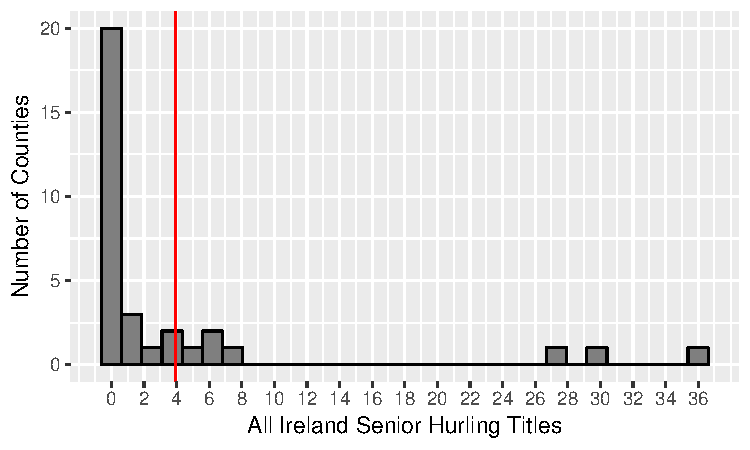
\includegraphics[width=.85\textwidth]{/Users/stefan/GitHub/po3600/plots/mt_01_hurling.pdf}
\end{figure}
\textbf{Top 3}: 1. Kilkenny (36); 2. Cork (30); 3. Tipperary (27)
\end{frame}

\begin{frame}{Distribution of All-Ireland Football Titles per County}

\begin{figure} \centering
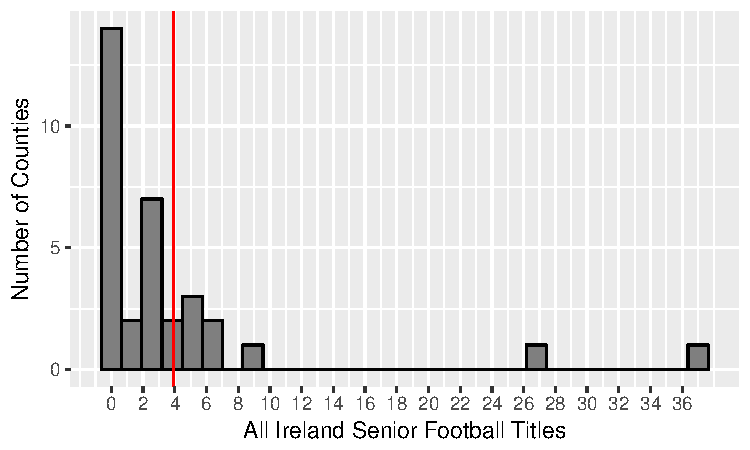
\includegraphics[width=.85\textwidth]{/Users/stefan/GitHub/po3600/plots/mt_01_football.pdf}
\end{figure}
\textbf{Top 3}: 1. Kerry (37); 2. Dublin (27); 3. Galway (9)
\end{frame}

\begin{frame}{Distribution of Bootstrapped Sample Means}

\begin{figure} \centering
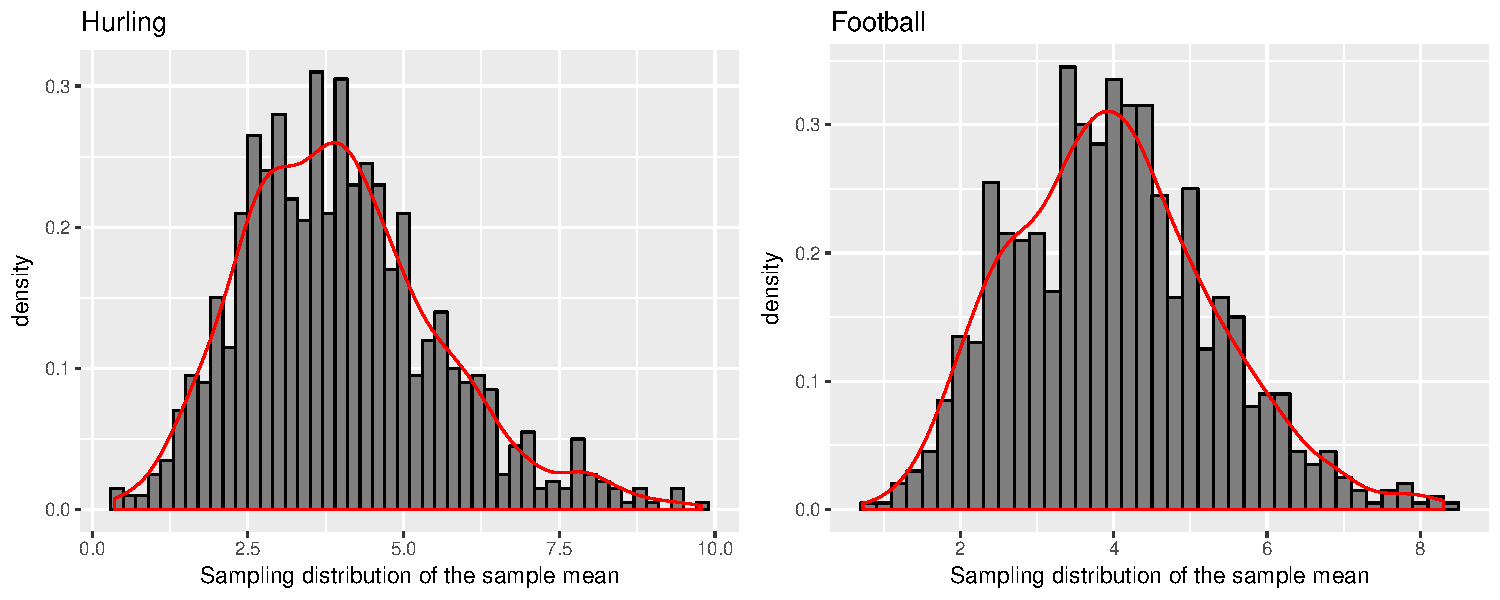
\includegraphics[width=1\textwidth]{/Users/stefan/GitHub/po3600/plots/mt_01_sampling_means.pdf}
\end{figure}
\textit{Note:} 1000 random draws, calculation of mean, plot of distribution; hypothetical example as we draw from the population!
\end{frame}


\section{How to Use SPSS}
\begin{frame}{SPSS}
\begin{itemize}
\item How to open (data) in SPSS?
\item How to work reproducibly in SPSS?
\end{itemize}
\end{frame}


\begin{comment}
\section{Discussion of Lecture Topics}
\begin{frame}{Central Terms and Definitions}

\begin{itemize}
\item Population
\item Sample
\item Random sample
\item Probability
\end{itemize}

\end{frame}

\begin{frame}{Central Terms and Definitions}

\begin{itemize}
\item Concept
\item Theory
\item Deduction
\item Induction
\item Levels of measurement: nominal, ordinal, interval-ratio
\end{itemize}

\end{frame}
\end{comment}



\end{document}